%\documentclass[11pt,professionalfonts,hyperref={pdftex,pdfpagemode=none,pdfstartview=FitH}]{beamer}
%\usepackage{times}
\documentclass[11pt,professionalfonts]{beamer}
\usefonttheme{serif}
\usepackage{presentation_packages}
\usepackage{animate} % for animated gif

\newcommand{\hilight}[1]{\colorbox{green}{#1}}

\definecolor{mygray}{gray}{0.9}
\definecolor{RoyalBlue}{rgb}{0.25,0.41,0.88}
\def\Emph{\textcolor{RoyalBlue}}

\definecolor{tmp}{rgb}{0.804,0.941,1.0}
\setbeamercolor{numerical}{fg=black,bg=tmp}
\setbeamercolor{exact}{fg=black,bg=red}

\mode<presentation> 
{
  \usetheme{Warsaw}
  \usefonttheme{serif}
  \setbeamercovered{transparent}
}

\setbeamertemplate{footline}%{split theme}
{%
  \leavevmode%
  \hbox{\begin{beamercolorbox}[wd=.5\paperwidth,ht=2.5ex,dp=1.125ex,leftskip=.3cm,rightskip=.3cm plus1fill]{author in head/foot}%
    \usebeamerfont{author in head/foot}\insertshorttitle
  \end{beamercolorbox}%
  \begin{beamercolorbox}[wd=.5\paperwidth,ht=2.5ex,dp=1.125ex,leftskip=.3cm,rightskip=.3cm]{title in head/foot}
%    \usebeamerfont{title in head/foot}\mypaper\hfill \insertframenumber/\inserttotalframenumber
    \usebeamerfont{title in head/foot}\hfill \insertframenumber/\inserttotalframenumber
  \end{beamercolorbox}}%
  \vskip0pt%
} \setbeamercolor{box}{fg=black,bg=yellow}


\title[Research Summary]{\large\bf  Research Summary}

\author{\vspace*{-0.3cm}}

%\institute{\footnotesize
%{\normalsize Shankar Kulumani}\vspace*{0.2cm}\\
%  Flight Dynamics and Control Lab \\ 
%  Dept. of Mechanical and Aerospace Engineering\\ 
%  The George Washington University \\
%  Washington, DC\\ \vspace{10pt}
%  June 4, 2014 \\ \vspace{10pt}
%  }
\date{29 September 2016}

\institute{
	\footnotesize
	{\normalsize\bf{Shankar Kulumani}}\\
	Ph.D. student\\
	\vspace*{0.2cm}
  	\bf{Department of Mechanical \& Aerospace Engineering}\\ \vspace*{0.5cm}
 	\begin{figure} %figure%
       	
\includegraphics[width=0.75\textwidth]{gw_txh_2cs_pos}
  	\end{figure}
}


\begin{document}
%=======================================================%

\setcounter{framenumber}{-1}
\begin{frame} %-----------------------------%
  \titlepage
\end{frame}   %-----------------------------%

\section{Low Thrust Transfers}
\subsection{Motivation}

\begin{frame}{Motivation} %--------------------------------------------------%
	\begin{itemize}
		\item Small satellites are more popular
		\begin{itemize}
			\item Reduced mass/size allows for efficient launch
			\item COTS components allows for standardization
		\end{itemize}
		\pause
		\item Low-thrust propulsion
		\begin{itemize}
			\item Minituarized electric propulsion systems
			\item Higher specific impulse
			\item Extended operating times 
		\end{itemize}
		\pause
		\item New mission types
		\begin{itemize}
			\item Spacecraft formations
			\item Orbital servicing
			\item Interplanetary swarms
		\end{itemize}
	\end{itemize}
	
\end{frame} %----------------------------------------------------------------%

\begin{frame} %-----------------------------%
\frametitle{Previous Work} % small satellites
\framesubtitle{Challenges}
\begin{itemize}
	\item Optimal Trajectory Design
		\begin{itemize}
			\item Orbital dynamics are nonlinear and chaotic
			\item Very sensitive to initial conditions
			\item Intuition required by designer
		\end{itemize}
	\pause
	\item Direct Optimal Control
		\begin{itemize}
			\item Reformulate problem as parameter optimization
			\item Allows for use of nonlinear programming methods
			\item High dimensional problem and computationally intensive
		\end{itemize}
	\pause
	\item Numerical Integration
		\begin{itemize}
			\item Typical methods use Runge-Kutta schemes
			\item Numerical Instability and Energy drift
			\item Difficult to capture  long-term effects of low-thrust propulsion accurately
		\end{itemize}
	\pause
	\item Invariant Manifolds
		\begin{itemize}
			\item Associated with periodic orbits
			\item Control-free and transfers require manifolds to intersect
		\end{itemize}
\end{itemize}
\end{frame}   %-----------------------------%

\begin{frame} % -----------------------------------%
\frametitle{Proposed Approach}
		\begin{itemize}
			\item Extend invariant manifold concept with low-thrust control  
			\item Variational integrator allows for accurate and stable computation
			\item \emph{Computational geometric optimal control}
			\begin{itemize}
				\item Generate the reachable set
			\end{itemize}
			\item \emph{Reachability set} on Poincar\'e section 
			\begin{itemize}
				\item Utilize a lower dimensional space allows for systematic transfer design
			\end{itemize}
		\end{itemize}
\end{frame} %--------------------------------------%

\subsection{Background}
% summary of three body problem
\begin{frame}
	\frametitle{PCRTBP}
	\begin{itemize}
		\item Motion of S/C under the influence of two attractive primaries
		\item EOMs - rotating reference frame and non-dimensionalized
	\end{itemize}
	\begin{figure}
		\centering
		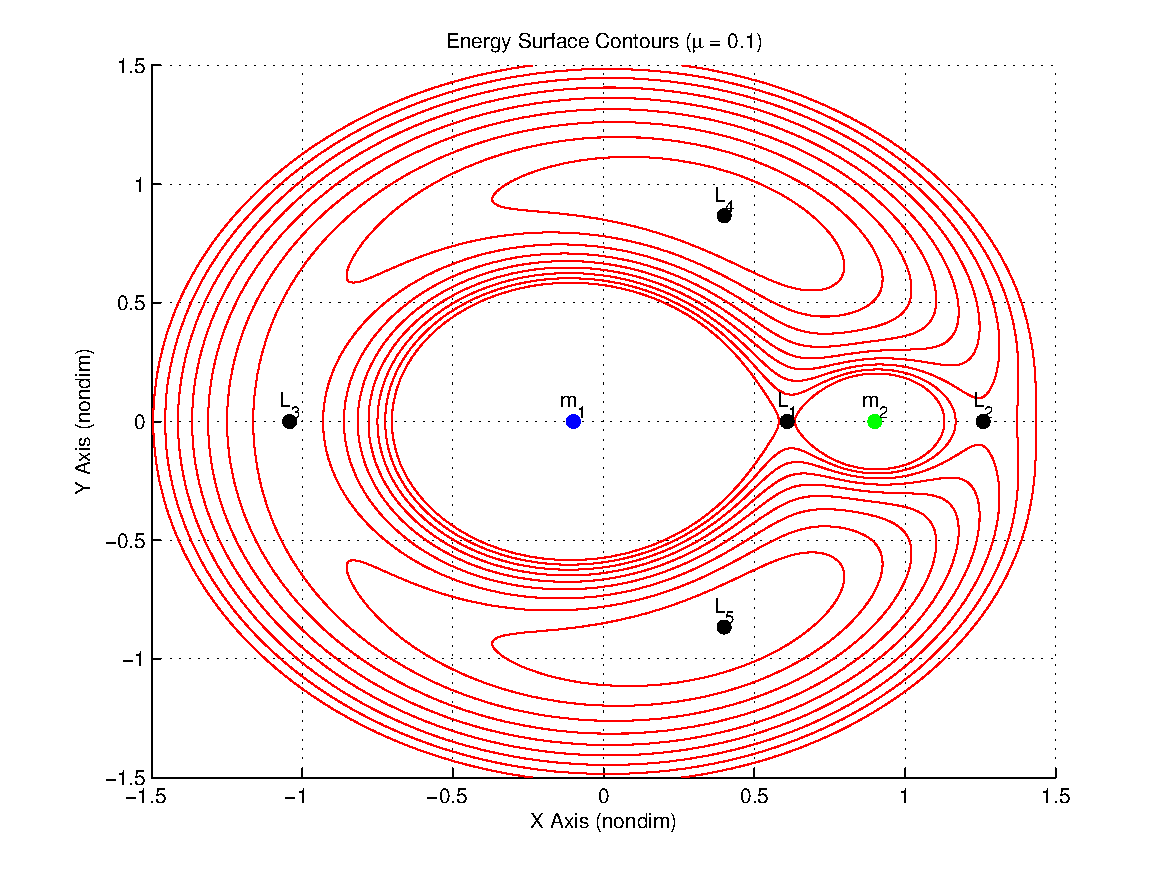
\includegraphics[height=0.7\textheight]{energy_contours}
	\end{figure}
	
\end{frame}

\begin{frame}{Invariant Manifolds} %----------------------------------------%
\begin{itemize}
	\item Sets of trajectories which asymptotically arrive and depart from a periodic orbit
	\item Allow for energy free transfers through configuration space
\end{itemize}
	\begin{figure}
		\centering
		\only<1>{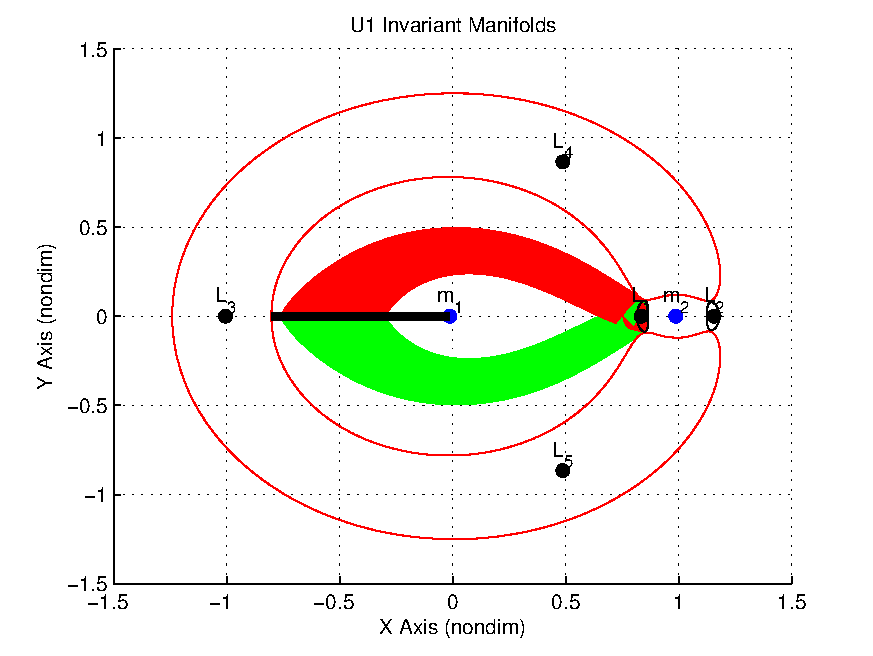
\includegraphics[height=0.7\textheight]{U1_Manifolds}}
		\only<2>{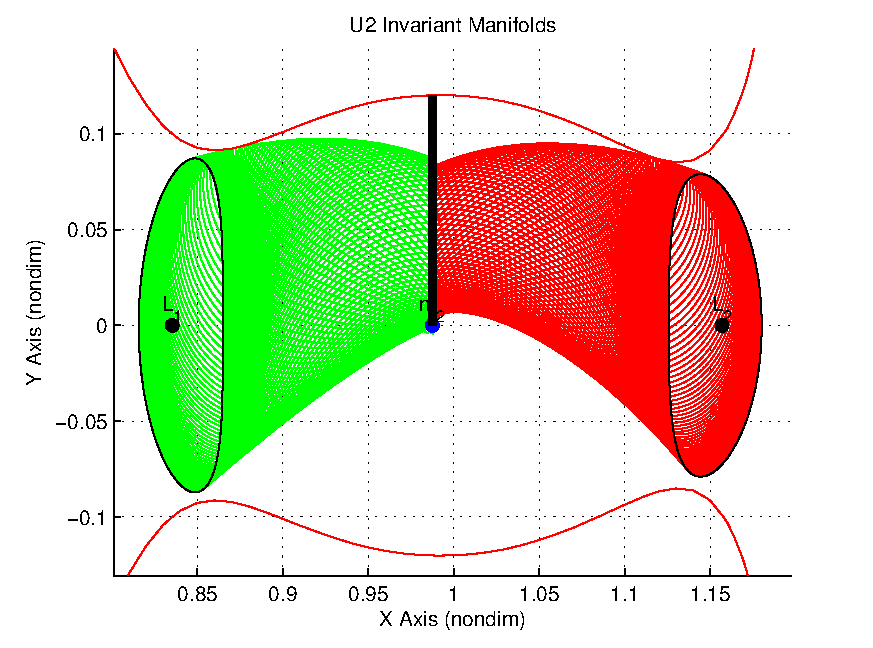
\includegraphics[height=0.7\textheight]{U2_Manifolds}}
		\only<3>{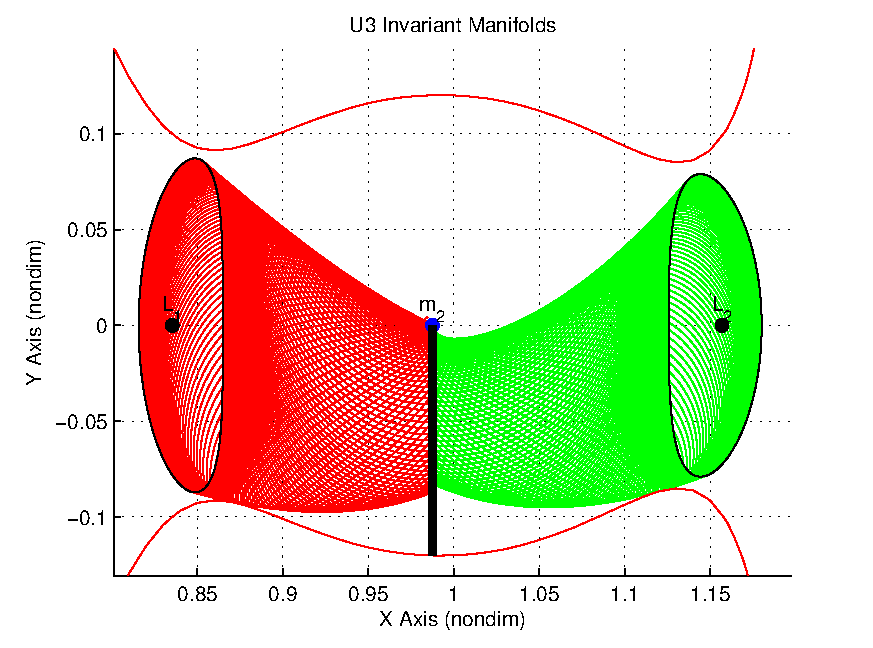
\includegraphics[height=0.7\textheight]{U3_Manifolds}}
		\only<4>{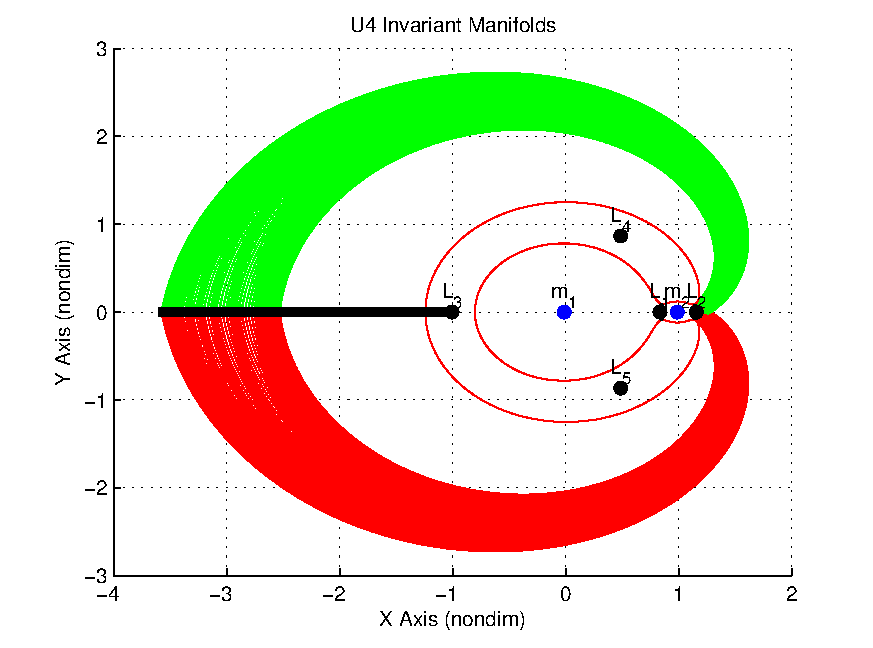
\includegraphics[height=0.7\textheight]{U4_Manifolds}}
	\end{figure}
\end{frame} %-------------------------------------------------%

\begin{frame}{\Poincare Section} %---------------------------------------%
\begin{itemize}
	\item Lower dimensional plane traverse to dynamic flow
	\item Analysis on a lower dimensional space
\end{itemize}
	\begin{figure}
		\centering
		\only<1>{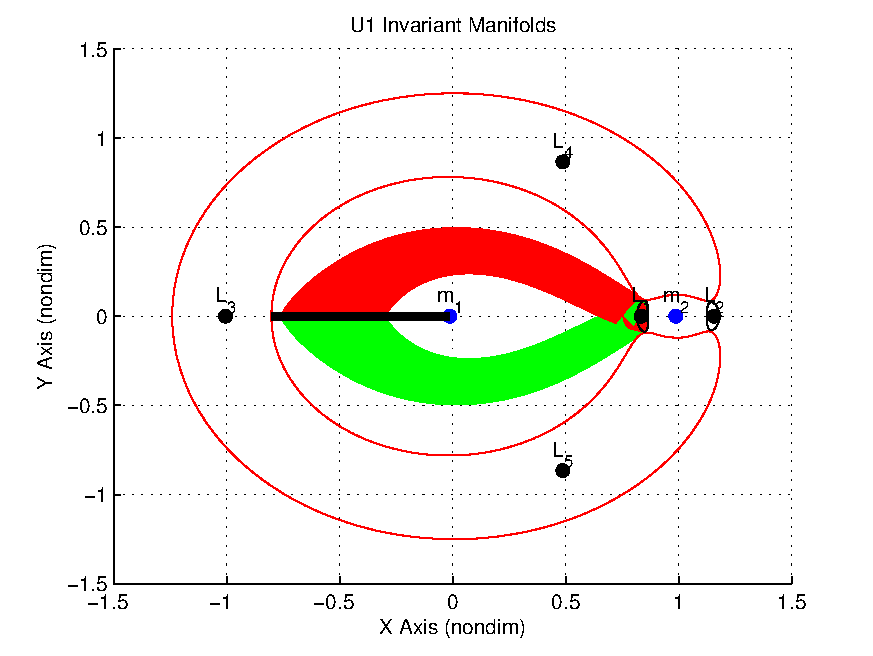
\includegraphics[height=0.4\textwidth]{U1_Manifolds}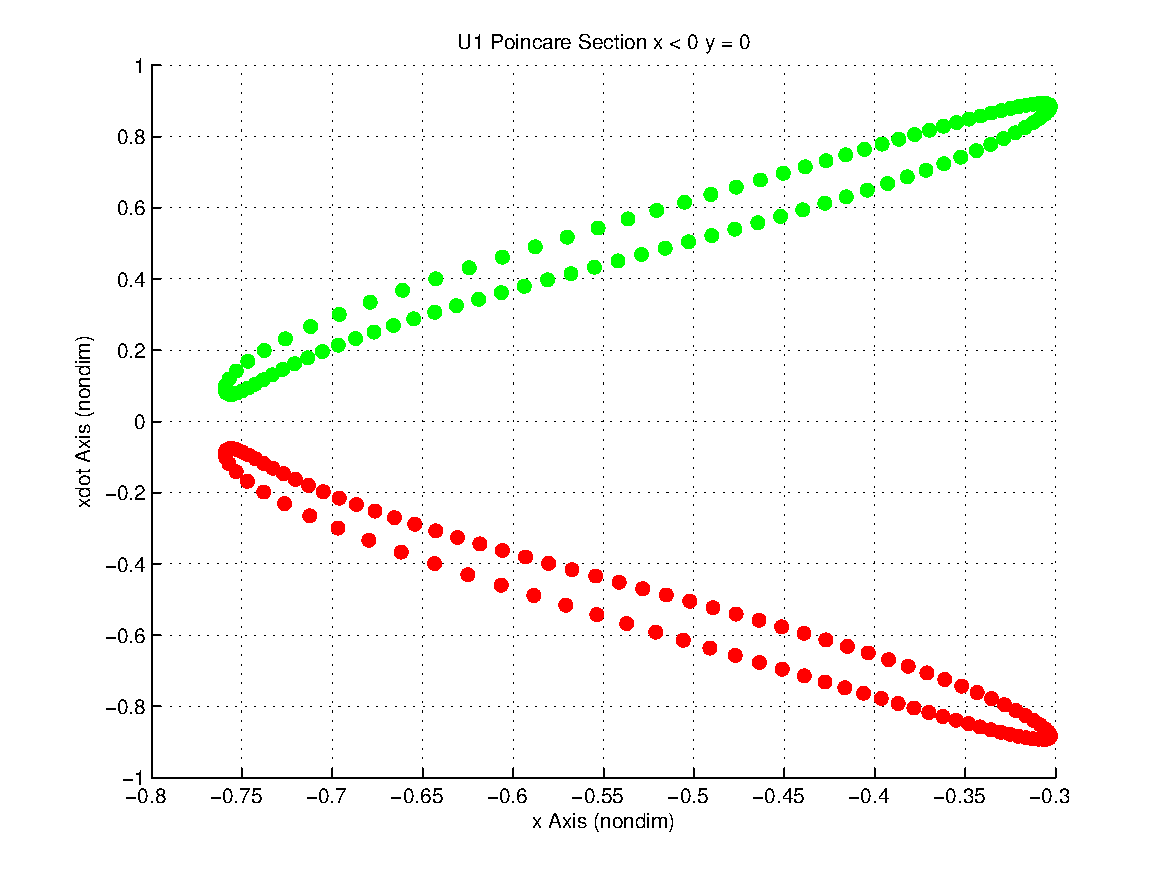
\includegraphics[height=0.4\textwidth]{U1_poincare}}
		\only<2>{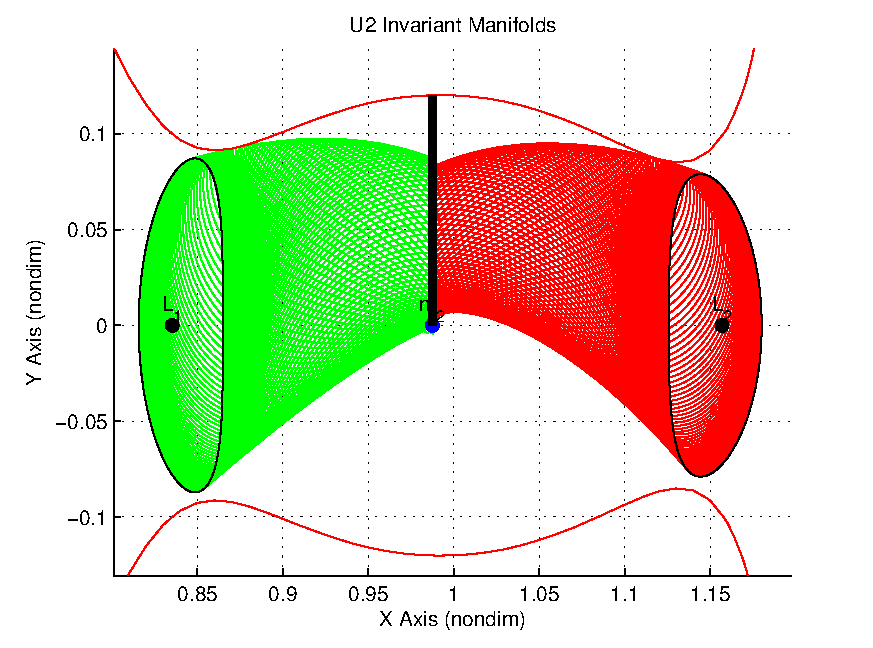
\includegraphics[height=0.4\textwidth]{U2_Manifolds}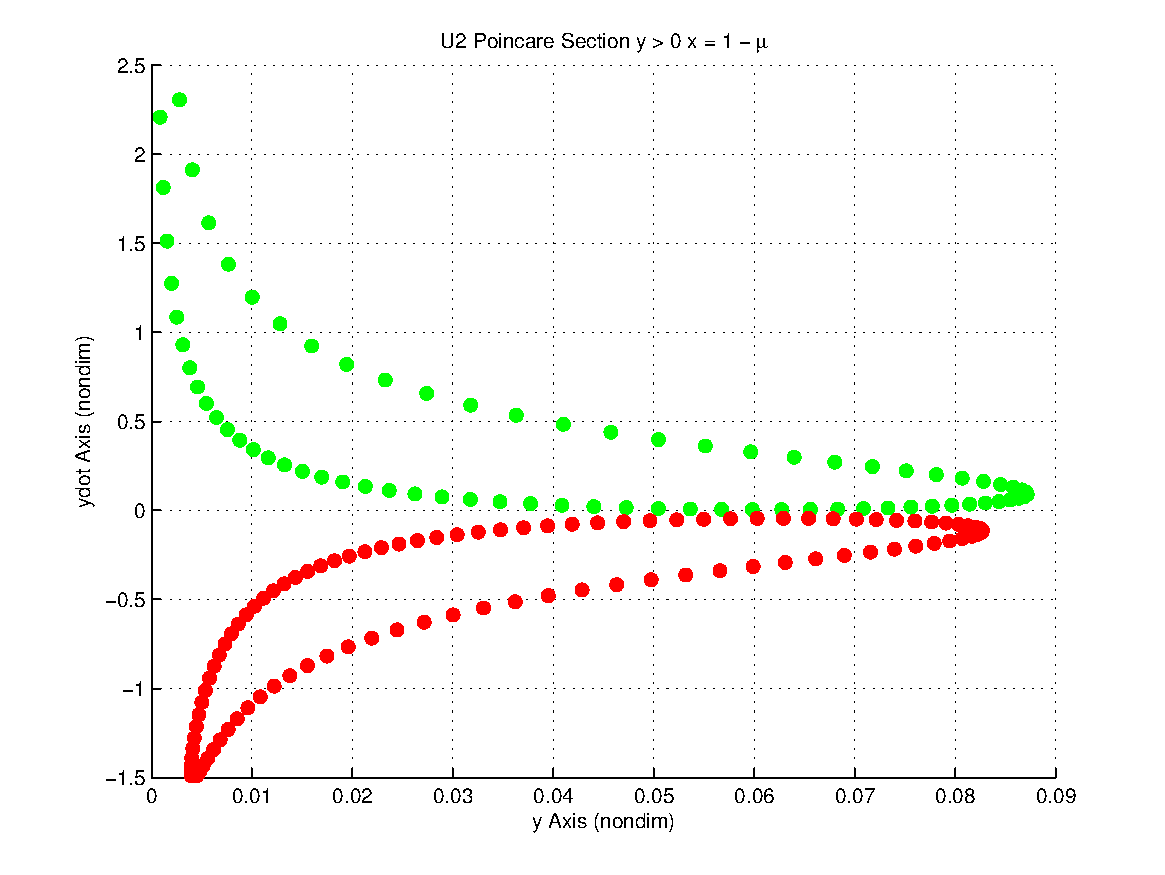
\includegraphics[height=0.4\textwidth]{U2_poincare}}
		\only<3>{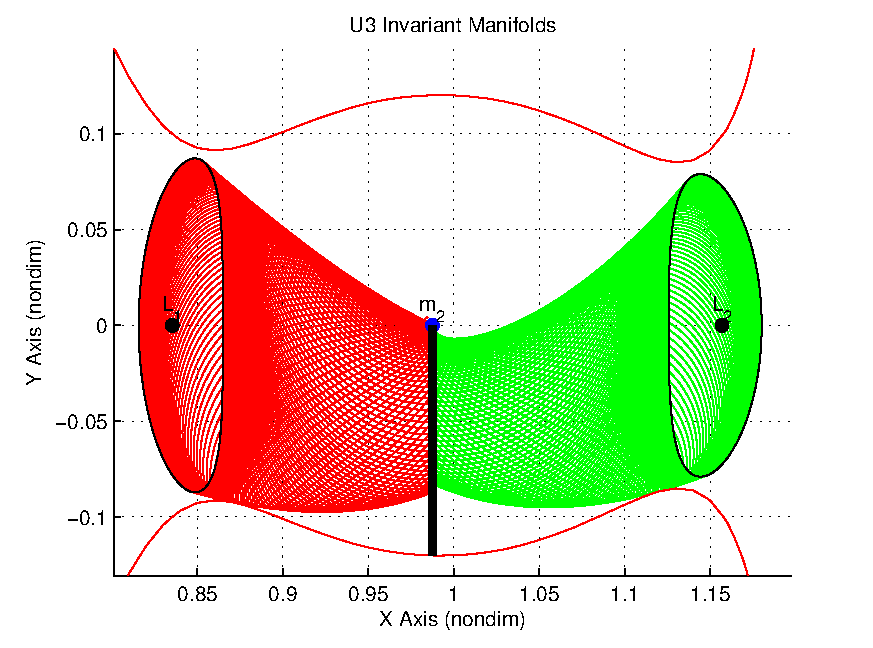
\includegraphics[height=0.4\textwidth]{U3_Manifolds}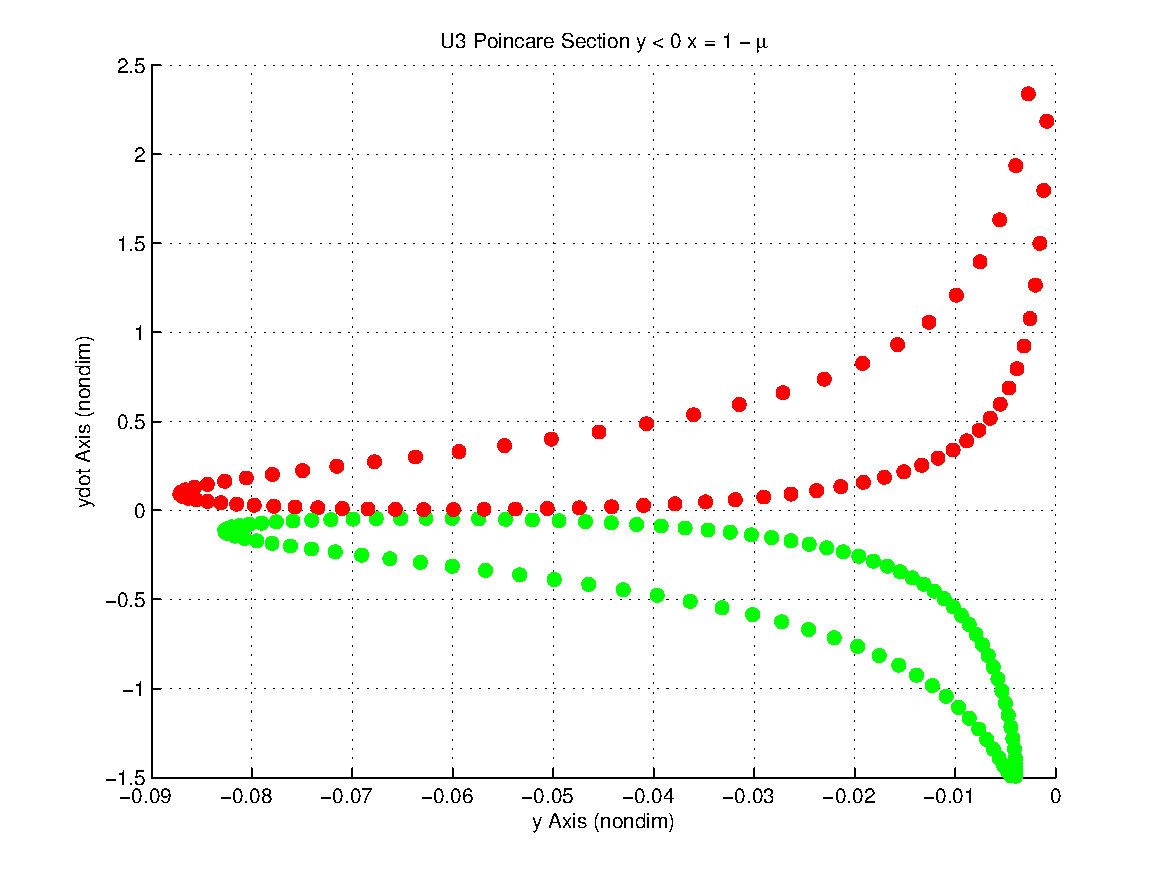
\includegraphics[height=0.4\textwidth]{U3_poincare}}
		\only<4>{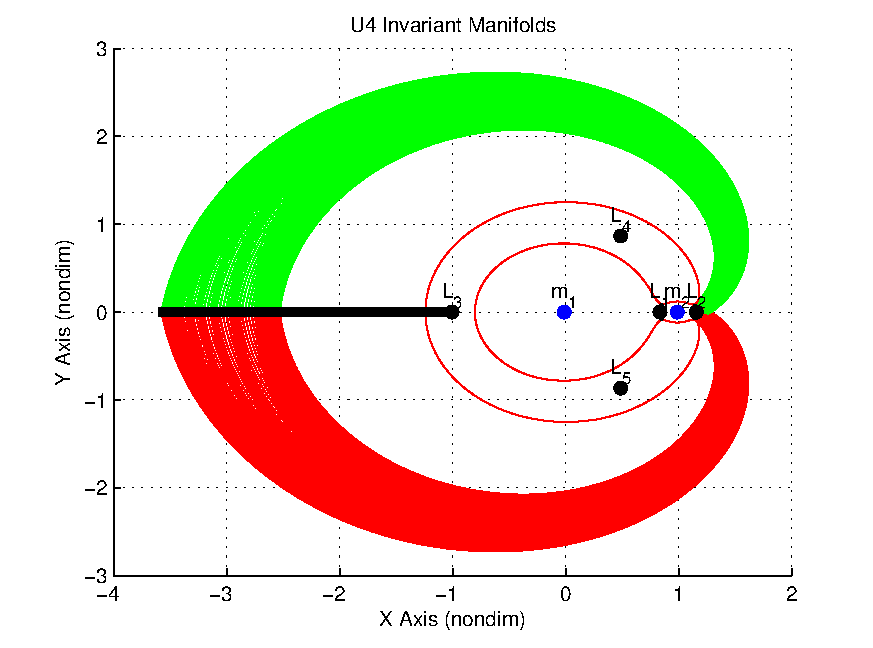
\includegraphics[height=0.4\textwidth]{U4_Manifolds}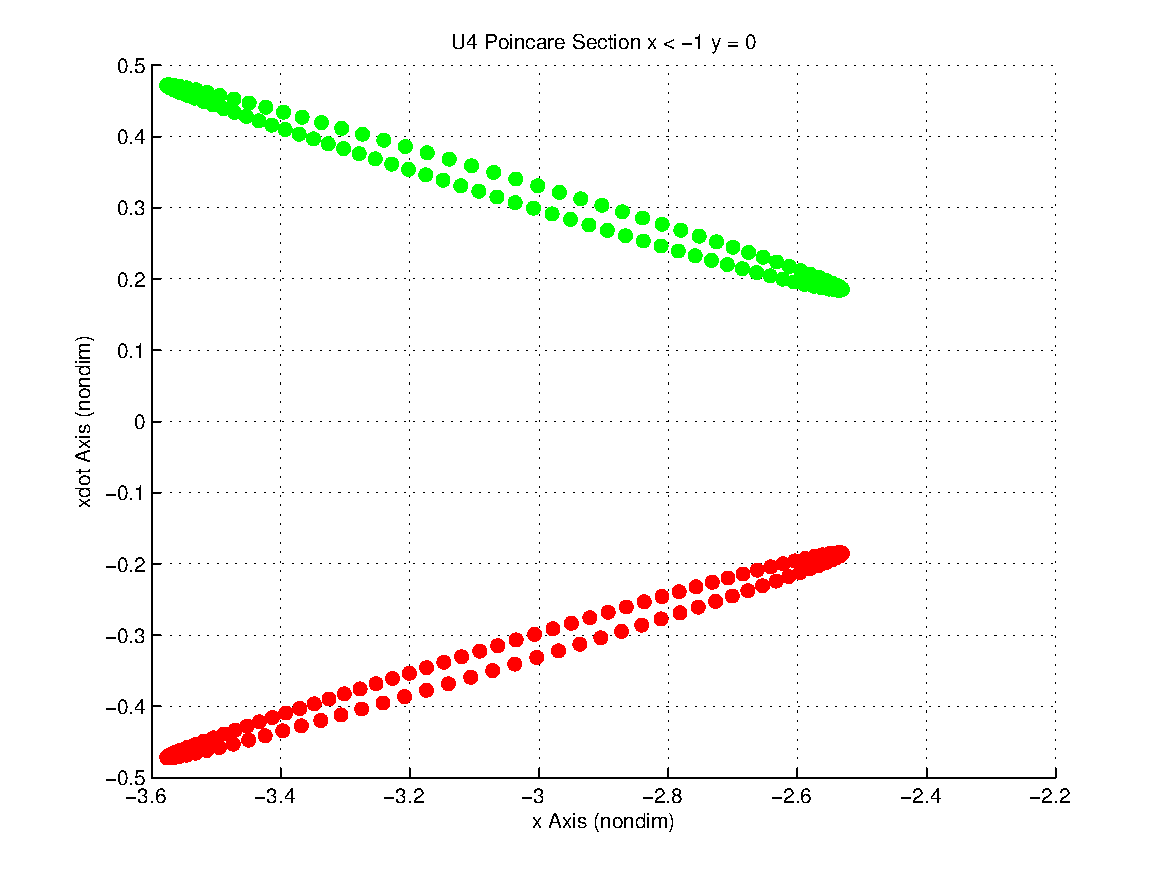
\includegraphics[height=0.4\textwidth]{U4_poincare}}
	\end{figure}
\end{frame} %--------------------------------------------%

%\begin{frame}[t] %---------------------------------------------------%
%\frametitle{Integrator Comparison}
%	\begin{itemize}
%		\item Numerical Simulation of PCRTBP (\( t_f = 200 \approx 15 \) years)
%			\begin{itemize}
%				\item Variable step Runge-Kutta method (\texttt{ode45.m})
%				\item Variational integrator \( \bar{x}_k \to \bar{x}_{k+1} \)
%			\end{itemize} 
%	\end{itemize}
%	\begin{figure} 
%	\centering 
%		\visible<2->{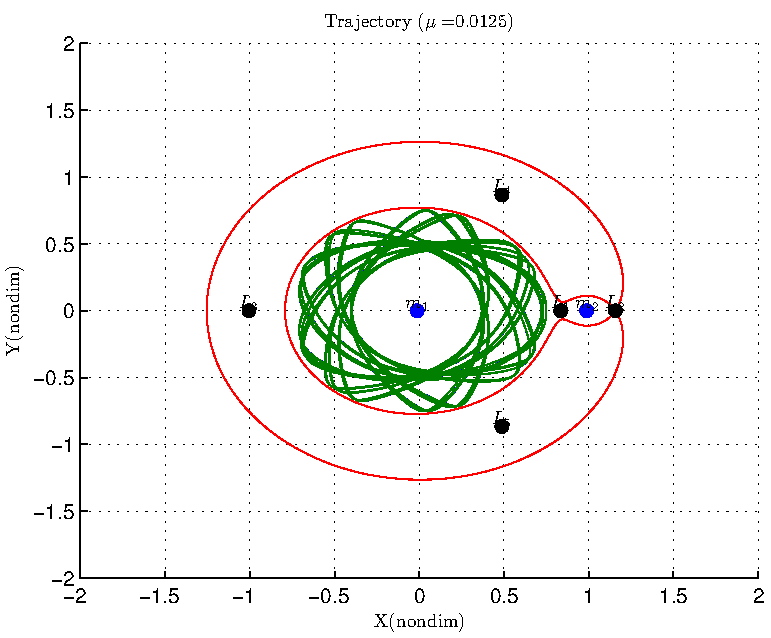
\includegraphics[width=0.5\textwidth]{./integrator_compare/trajectory}}% 
%		\visible<2->{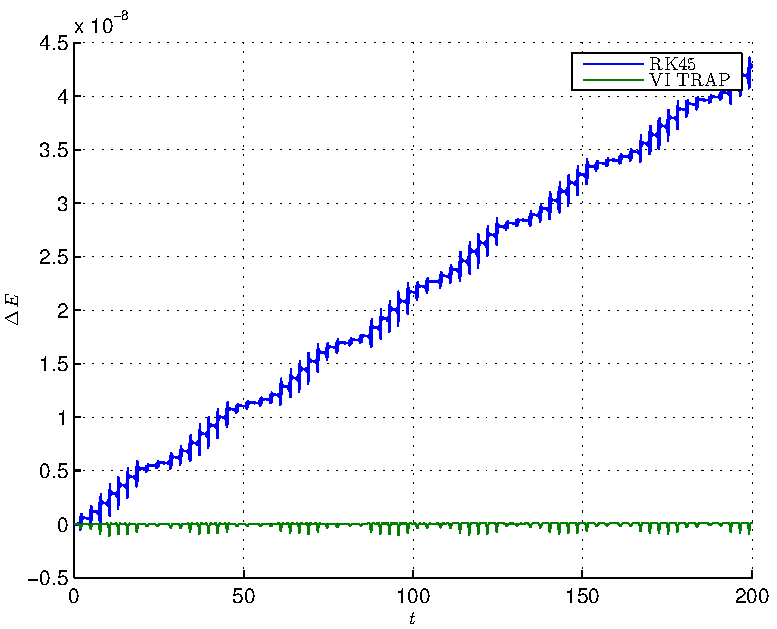
\includegraphics[width=0.5\textwidth]{./integrator_compare/energy} }
%	\end{figure}
%	
%	\begin{itemize}
%		\visible<2->{\item Typical integration methods do not preserve structure}
%	\end{itemize}
%\end{frame} %------------------------------------------------------%

%\begin{frame}[t]%---------------------------------------%
%\frametitle{Poincar\'e Section}
%	\begin{itemize}
%		\item Define hyperplane transverse to dynamic flow
%		\item Analysis on a lower dimensional space
%	\end{itemize}
% \begin{figure}
%     \centering
%     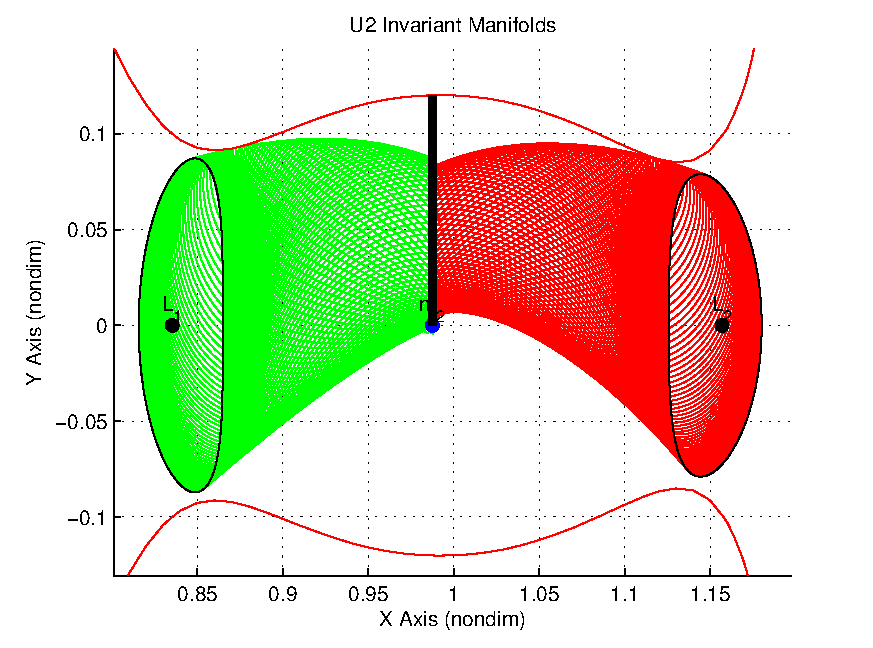
\includegraphics[width=0.5\columnwidth]{U2_Manifolds}%
%     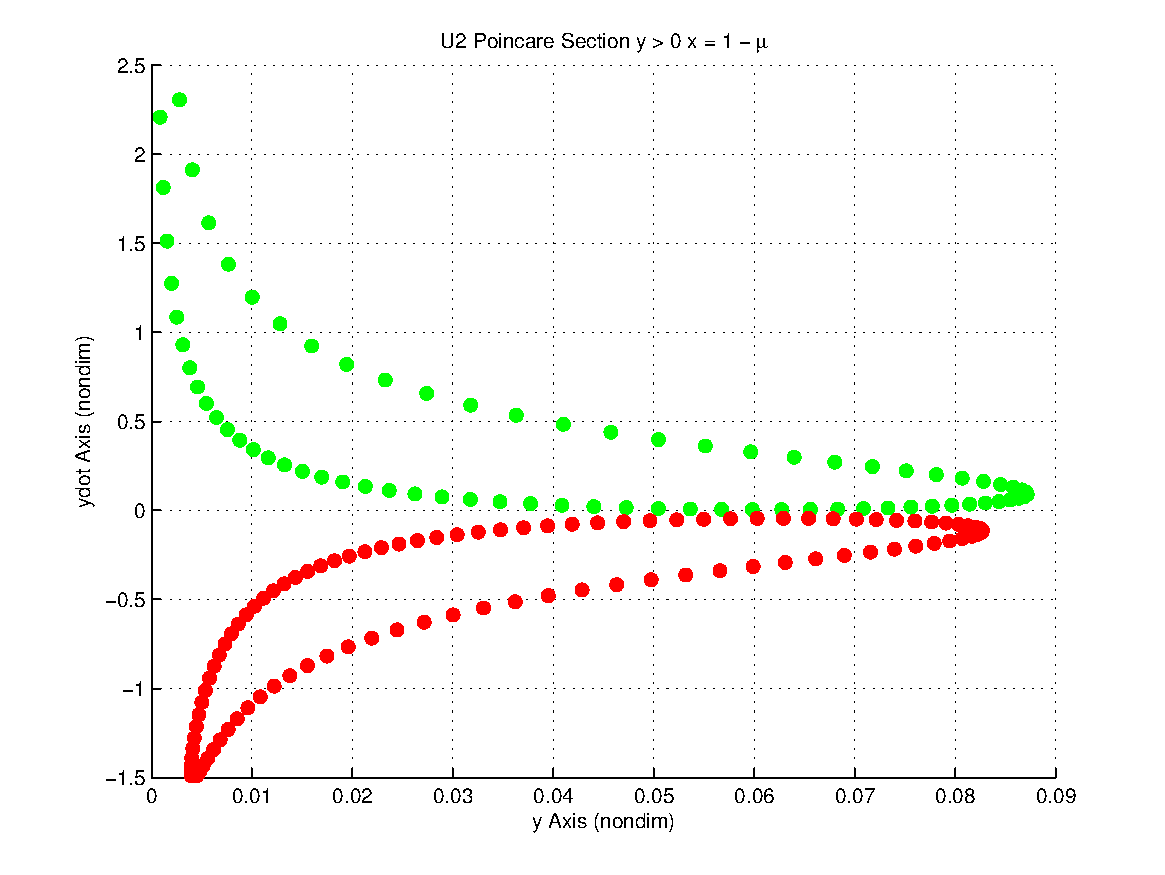
\includegraphics[width=0.5\columnwidth]{U2_poincare}
%\end{figure}
%
%	\pause
%	\begin{itemize}
%		\item Transfer is limited to intersecting regions
%	\end{itemize}
%	
%	\note[itemize]{
%		\item Lower state space from 4D to 2D
%		\item Energy Constant and Poincar\'e section plane are two constraints which reduce the state space
%		\item Extend invariant manifold transfer concept with addition of control input
%	}
%\end{frame}%--------------------------------%

\begin{frame} %------------------------------------%
\frametitle{Variational Principle}
	\begin{itemize}
		\item Variational Integrators
			\begin{itemize}
				\item Structure-preserving integrators for Hamiltonian systems
				\item Obtained by discretizing variational principle
			\end{itemize}
	\end{itemize}
	\pause
	\begin{columns}[c]
		\begin{column}{0.5\textwidth}
			\centering
			\begin{beamercolorbox}[wd=0.8\columnwidth,sep=0.05cm,center]{numerical} Continuous Time \end{beamercolorbox}
			\begin{beamercolorbox}[wd=0.8\columnwidth,sep=0.05cm,center]{numerical} 
				Configuration Space \\
				\( \parenth{q, \dot{q} } \in TQ \)
			\end{beamercolorbox}
			\begin{beamercolorbox}[wd=0.8\columnwidth,sep=0.05cm,center]{numerical} 
				Lagrangian \\
				\( L\parenth{q, \dot{q} } \)
			\end{beamercolorbox}
			\begin{beamercolorbox}[wd=0.8\columnwidth,sep=0.05cm,center]{numerical} 
				Action Integral \\
				\( S = \int_{0}^T L\left( q, \dot{q}\right) \, dt \)
			\end{beamercolorbox}
			\begin{beamercolorbox}[wd=0.8\columnwidth,sep=0.05cm,center]{numerical} 
				Stationary Action \\
				\( \delta S = 0 \)
			\end{beamercolorbox}
%			\begin{beamercolorbox}[wd=0.8\columnwidth,sep=0.05cm,center]{numerical} 
%				Legendre Transform \\
%				\( p_i = \deriv{L}{\dot{q}} \)
%			\end{beamercolorbox}
			\begin{beamercolorbox}[wd=0.8\columnwidth,sep=0.05cm,center]{numerical} 
				Equation of Motion \\
				\( \ddot{q} = f \parenth{q, \dot{q} } \)
			\end{beamercolorbox}
		\end{column}
		\pause
		\begin{column}{0.5\textwidth}
			\centering
			\begin{beamercolorbox}[wd=0.8\columnwidth,sep=0.05cm,center]{numerical} Discrete Time \end{beamercolorbox}
			\begin{beamercolorbox}[wd=0.8\columnwidth,sep=0.05cm,center]{numerical} 
				Configuration Space \\
				\( \parenth{q_k, q_{k+1} } \in Q \times Q \)
			\end{beamercolorbox}
			\begin{beamercolorbox}[wd=0.8\columnwidth,sep=0.05cm,center]{numerical} 
				Lagrangian \\
				\( L_d\parenth{q_k, q_{k+1}} \)
			\end{beamercolorbox}
			\begin{beamercolorbox}[wd=0.8\columnwidth,sep=0.05cm,center]{numerical} 
				Action Sum \\
				\( S_d = \sum_{k=0}^{N-1} L_d(q_k, q_{k+1}) \)
			\end{beamercolorbox}
			\begin{beamercolorbox}[wd=0.8\columnwidth,sep=0.05cm,center]{numerical} 
				Stationary Action \\
				\( \delta S_d = 0 \)
			\end{beamercolorbox}
%			\begin{beamercolorbox}[wd=0.8\columnwidth,sep=0.05cm,center]{numerical} 
%				Fiber Derivative \\
%				\( p_k = - \deriv{L_d(q_k, q_{k+1})}{q_k} \) \\
%				\( p_{k+1} = \deriv{L_d(q_k, q_{k+1})}{q_{k+1}} \)
%			\end{beamercolorbox}
			\begin{beamercolorbox}[wd=0.8\columnwidth,sep=0.05cm,center]{numerical} 
				Equation of Motion \\
				\( q_{k+2} = f_d \parenth{q_k, q_{k+1} } \)
			\end{beamercolorbox}
		\end{column}
	\end{columns}
	
	\note[itemize]{
		\item Continous time - discretization occurs at end while implemented in digital computer
		\item Discrete time - discretization occurs at the beginning. 
		Dynamics derived in discrete time
		\item Legendre transform allows for expression of dynamics in Hamiltonian form
	}
\end{frame}%-----------------------------------------%


\subsection{Research}
\begin{frame} %-----------------------------%
\frametitle{Reachability Set}
  \begin{itemize}
  \item Reachable set on Poincar\'e section
  		\begin{itemize}
  			\item The set of states that can be attained from a given initial state via admissable control input
  			\item Enlarge the intersection region on the Poincar\'e section
  		\end{itemize}
  \item \emph{Computational Geometric Optimal Control}
	\begin{itemize}
  		\item Poincar\'e section defined by \( \alpha_d \) in \( m_1\)
		\item Direction on Poincar\'e section defined by \( \theta_d \) in \( m_2 \)
	\end{itemize}
 \end{itemize}
  \begin{align*}
	J &= -\frac{1}{2} \left( \bar{x}(N) - \bar{x}_{n}(N)\right)^T Q_f\left( \bar{x}(N) - \bar{x}_{n}(N)\right)\\
	m_1 &= 0 = \frac{y(N) - L_{1y}}{x(N) - L_{1x}} - \tan{\alpha_d} \\ 
    m_2&= 0 = \frac{\dot{x}(N) - \dot{x_n}(N) }{x(N) -x_n(N) } - \tan{\theta_d} \\
	 0 &\geq\bar{u}^T \bar{u} - u_{max}^2 
	\end{align*}

	\note[itemize]{
		\item E-L equations are used to derive necessary conditions for optimality
		\item Results in TPBVP and indirect optimal control
		
	}
\end{frame}   %-----------------------------%

\begin{frame} %-----------------------------------------------%
\frametitle{Invariant Manifold Transfer}
\begin{itemize}
	\item Unstable invariant manifolds generated from periodic orbit
	\item Poincar\'e section intersections generated
\end{itemize}
	\begin{figure} 
	\centering 
	\begin{subfigure}[htbp]{0.5\textwidth} 
		\visible<2->{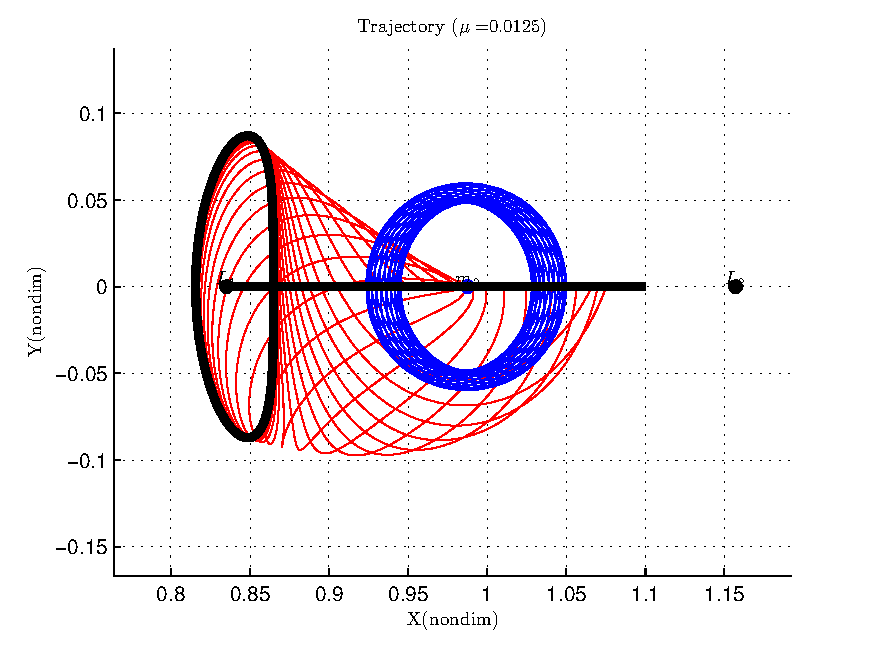
\includegraphics[width=\textwidth]{manifold_trajectory}  }
	\end{subfigure}~
	\begin{subfigure}[htbp]{0.5\textwidth} 
		\visible<3->{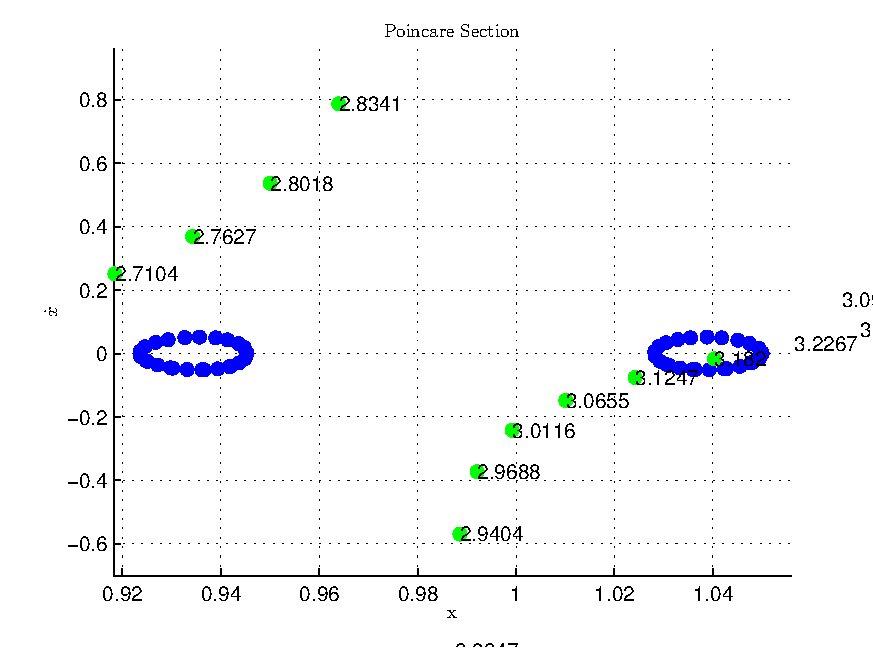
\includegraphics[width=\textwidth]{manifold_poincare} }
	\end{subfigure} 
	\end{figure}
	\visible<4->{
	\begin{itemize}
		\item Only portion of invariant manifold intersects the target
		\item Long time of flight \( t_f \approx 3.1 \)
	\end{itemize}
	}
	\note[itemize]{
		\item Show invariant manifold transfer
		\item Discuss how manifold sometimes don't intersect
		\item Also has a long time of flight
		\item Manifolds are generated using a linear analysis.
		Eigenvectors are local approximation of stable/unstable directions
		Perturb in direction of eigenvector then propogate to Poincar\'e section
		}
\end{frame} %------------------------------------------------%

\begin{frame}%------------------------------------------------%
\frametitle{Reachable Set Transfer}
\begin{itemize}
	\item Reachablility set generated on Poincar\'e section
	\item<3-> Intersection point used to generate a transfer
\end{itemize}
	\begin{figure} 
	\centering 
	\begin{subfigure}[htbp]{0.5\textwidth} 
		\only<1-2>{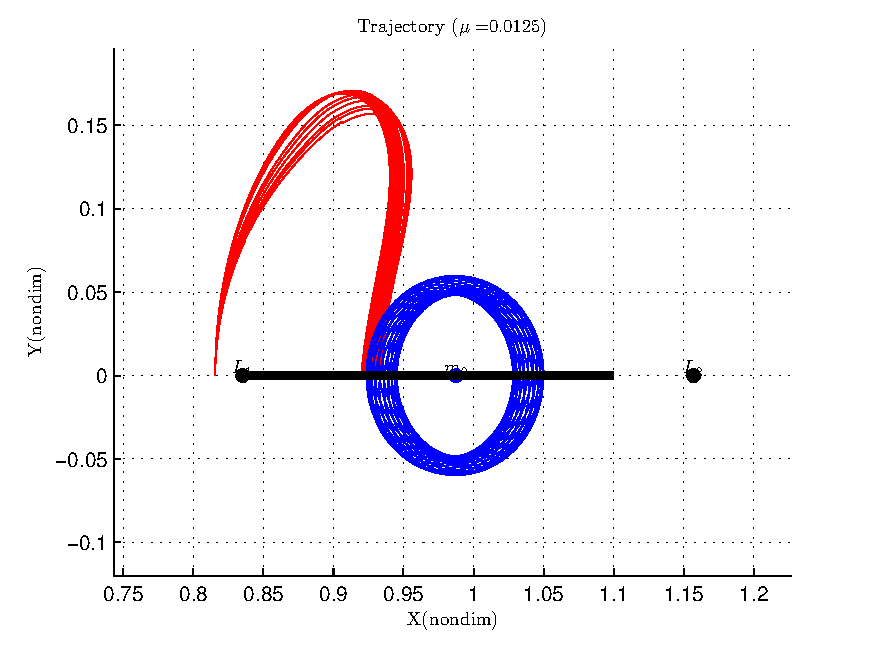
\includegraphics[width=\textwidth]{reach_trajectory}  }
		\visible<3->{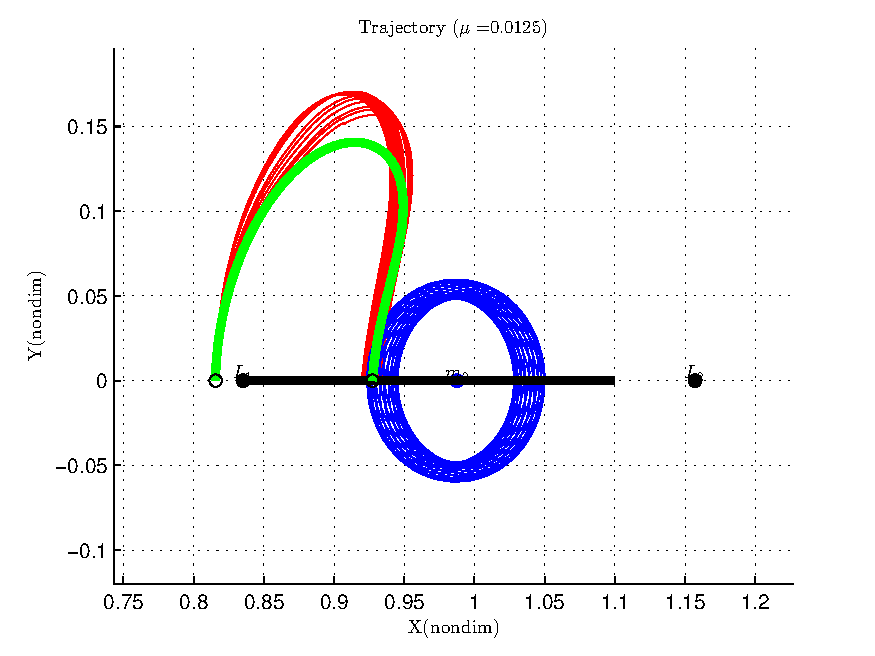
\includegraphics[width=\textwidth]{reach_transfer}  }
	\end{subfigure}~
	\begin{subfigure}[htbp]{0.5\textwidth} 
		\visible<2->{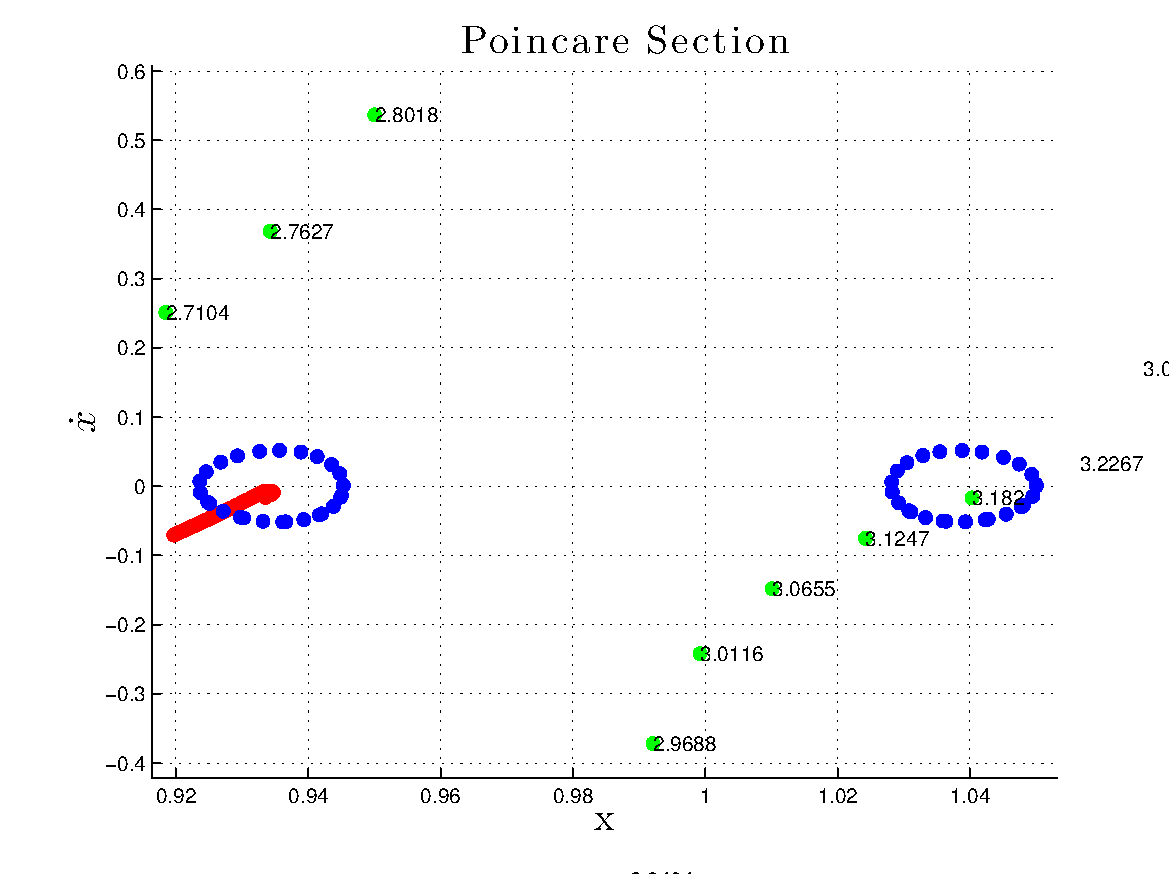
\includegraphics[width=\textwidth]{poincare_compare} }
	\end{subfigure} 
	\end{figure}
	
		\visible<4->{
	\begin{itemize}
		\item  Reachable set intersect the target 
		\item Shorter time of flight \( t_f \approx 1.4 \)
	\end{itemize}
	}
	\note[itemize]{
		\item Compare to reachable set approach
		\item Shorter time of flight
		\item Multiple shooting to solve TPBVP
		Vary \( \theta\) to change direction on section
		Linear interpolation to determine intersection on Poincar\'e section
		}
\end{frame} %--------------------------------------------------%

\begin{frame}{Geostationary to \( L_1 \) transfer} %----------------------------------------------------%
\begin{itemize}
	\item Tranfer for geostationary orbit to a periodic orbit about \( L_1\)
	\item Multiple iterations of reachable set
\end{itemize}

\begin{figure} 
	\centering 
	\begin{subfigure}[htbp]{0.5\textwidth} 
		\only<1>{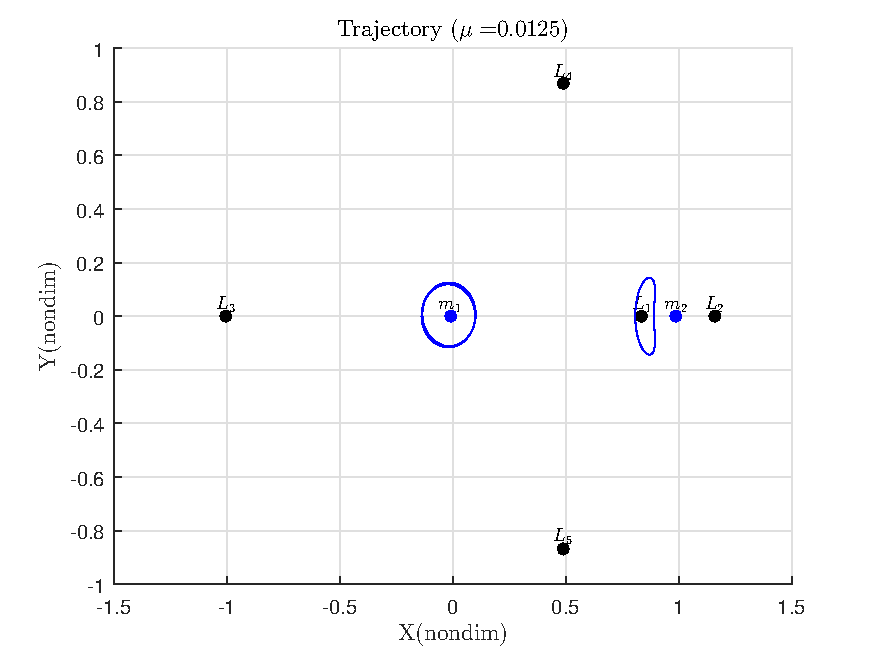
\includegraphics[width=\textwidth]{initial_final}  }
		\only<2>{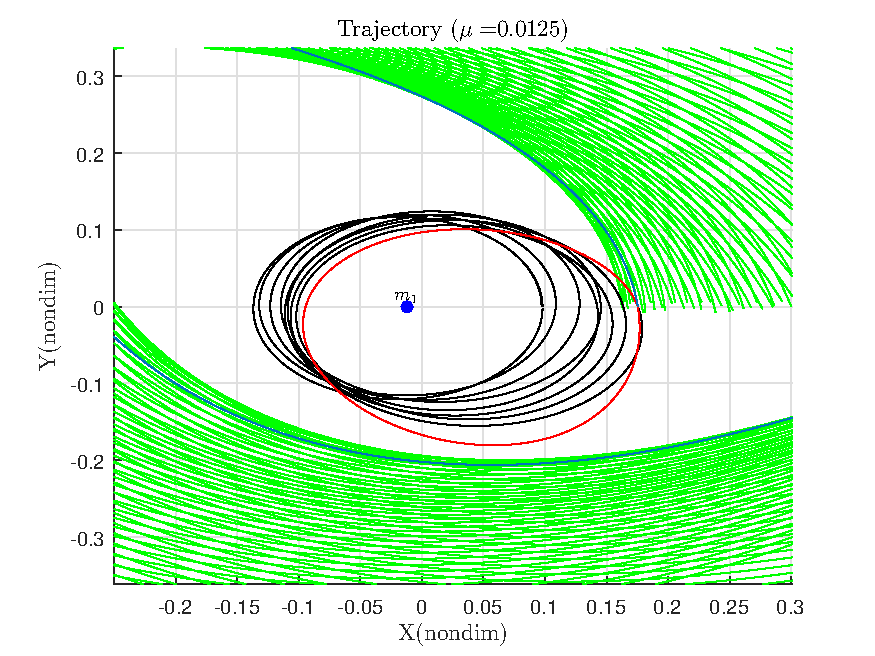
\includegraphics[width=\textwidth]{geo_transfer_zoom}  }
	\end{subfigure}~
	\begin{subfigure}[htbp]{0.5\textwidth} 
		\only<1>{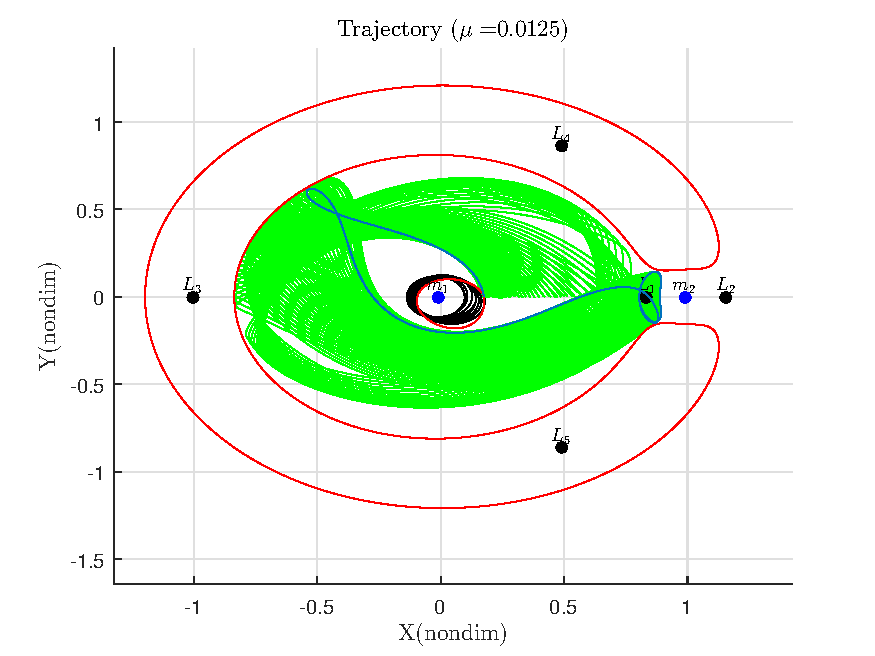
\includegraphics[width=\textwidth]{geo_transfer_full} }
		\only<2>{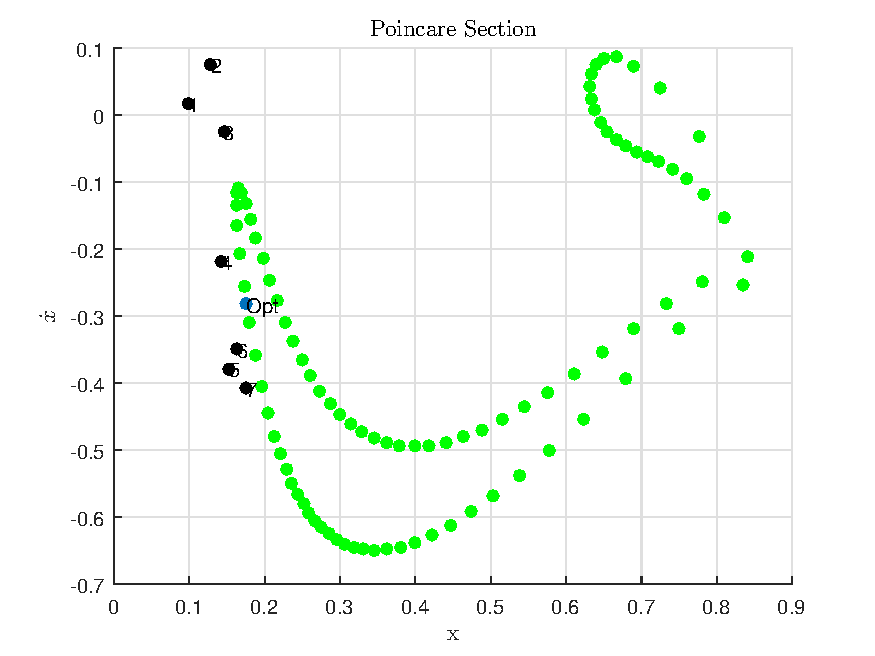
\includegraphics[width=\textwidth]{poincare}}
	\end{subfigure} 
	\end{figure}

\end{frame} %--------------------------------------------%


\section{Constrained Attitude Control}
\subsection{Motivation}

\begin{frame} %--------------------------------%
	\frametitle{Motivation}
	\begin{itemize}
		\item Constrained rigid body attitude control
		\begin{itemize}
			\item Examples: spacecraft and robotic vehicles
			\item Attitude constraints: exposure concerns for optical payloads
			\begin{itemize}
				\item Bright objects: Sun, Moon
				\item Incoming debris
				\item Hostile action: directed energy
			\end{itemize}
		\end{itemize}
	\pause
	\item Previous approaches have several issues
	\begin{itemize}
		\item Attitude parameterizations: singularities/ambiguities
		\item Ad-hoc geometric approach: find intermediate points
		\item Randomized methods: stochastic stability result
		\item Barrier function: Motion planning/Optimal Control
	\end{itemize}
\end{itemize}
\end{frame} %----------------------------------%

\begin{frame}{Attitude Parameterizations}
	\begin{itemize}
		\item Euler Angles
		\begin{itemize}
			\item Minimal representation used for small attitude changes.
			\item Singularities exist for large angle slews: requires switching between 24 sequences
			\item Complicated trigonometric functions
		\end{itemize}
		\pause
		\item Quaternion 
		\begin{itemize}
			\item No singularities
			\item Two anti-podal quaternions for the same attitude
			\item Unwinding behavior 
		\end{itemize}
		\pause
		\item Geometric control
		\begin{itemize}
			\item Globally and uniquely characterize attitude: \( R \in \SO \)
			\item Singular representation of attitude 
			\item Geometrically exact
		\end{itemize}
	\end{itemize}
	
\end{frame}

\subsection{Research}

\begin{frame}{Research Objectives}
\begin{itemize}
	\item Attitude manuevers with state inequality constraints
	\item Barrier function approach on \( \SO \) 
	\begin{itemize}
		\item Aggressive, global manuevers free from singularities
	\end{itemize}
	\item Mathematically rigorous stability guarantee
\end{itemize}
\end{frame}

\begin{frame} %-----------------------------%
\frametitle{Attitude dynamics} 
\begin{itemize}

	\item Configuration space: rotation matrix from body frame to inertial frame
	 \[\SO =  \{R\in\R^{3\times 3}\,|\, R^TR=I,\;\mathrm{det}[R]=1\} \]
	\item Rigid body attitude dynamics:
\begin{gather*}
	J\dot\Omega + \Omega\times J\Omega = u+W(R,\Omega)\Delta \\
	\dot R = R\hat\Omega 
\end{gather*}
\end{itemize}

\end{frame}   %-----------------------------%

\begin{frame}{Constraints} %-------------------------------------------%
	\begin{itemize}
		\item Body fixed vector \( r \in \S^2\) - a light sensitive optical sensor
		\item Inertially fixed vector \( v \in \S^2 \) - bright object 
		\item Hard cone constraint:
		\[
			r^T R^T v \leq \cos \theta
		\]
	\end{itemize}
	\pause
	\begin{block}{Control Design Goal}
		Design control input \( u \) that stabilizes system from initial attitude \( R_0 \) to desired attitude \( R_d \) while satisfying constraint.
	\end{block}
\end{frame}%-------------------------------------%

\begin{frame}%-----------------------------------------------------%
\frametitle{Configuration Error Function}
\begin{itemize}
	\item Configuration error function used to quantify attitude error
        \[
        	\Psi(R) = A(R) B(R) 
        \]
	\item Combination of attractive and repulsive terms   
        \begin{gather*}
        	A(R) = \frac{1}{2} \tr{G \left( I - R_d^T R\right)} \\
        	B_i(R) = 1 - \frac{1}{\alpha_i} \ln \left( - \frac{ r^T R^T v_i - \cos \theta_i}{1 + \cos \theta_i}\right)
        \end{gather*}
\end{itemize}
\visible<2->{
\begin{figure} 
	\centering 	
	\begin{subfigure}[b]{0.3\textwidth} 
		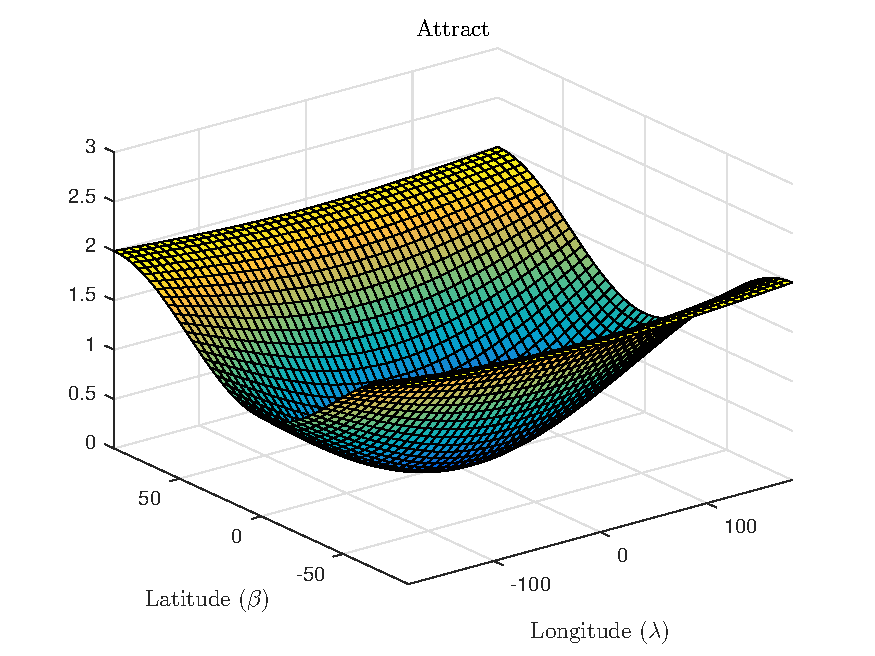
\includegraphics[width=\textwidth]{attract_error}
	\end{subfigure}~
	\begin{subfigure}[b]{0.3\textwidth} 
		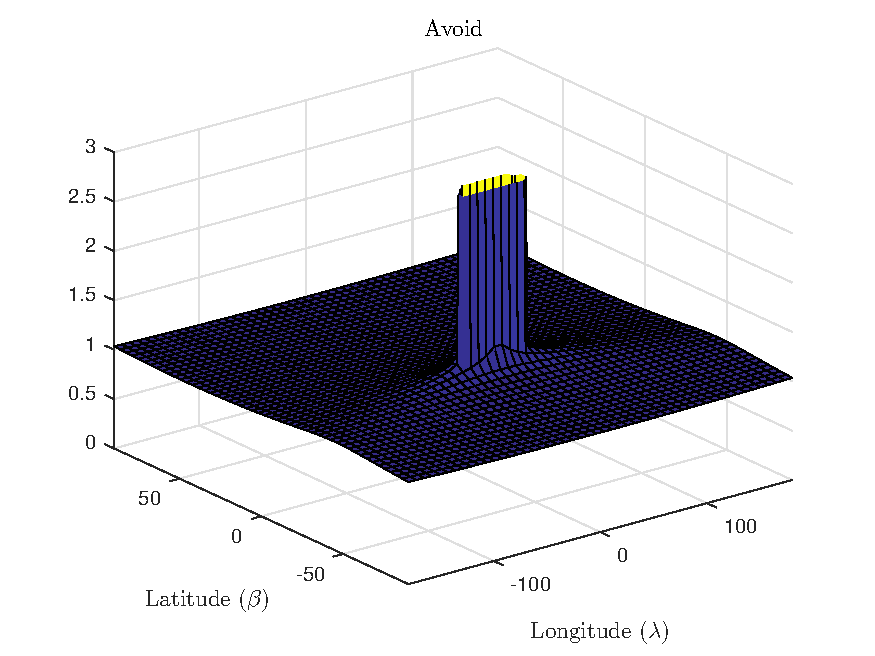
\includegraphics[width=\textwidth]{avoid_error}
	\end{subfigure}~
	\begin{subfigure}[b]{0.3\textwidth} 
		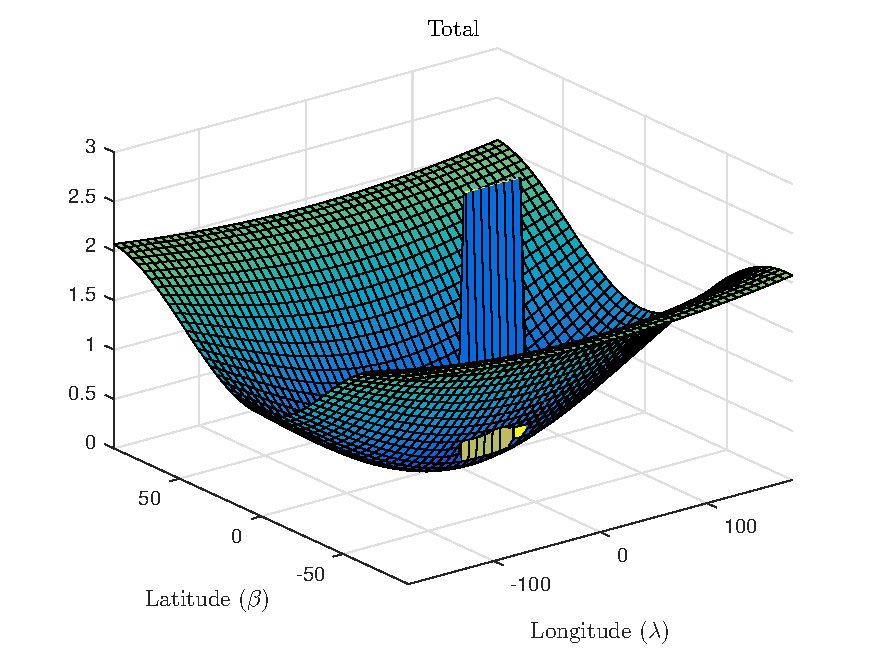
\includegraphics[width=\textwidth]{combined_error}
	\end{subfigure}
\end{figure}
}
\end{frame} %---------------------------------------------------%

\begin{frame}{Controller Design} %--------------------------------------------%
	\begin{block}{Adaptive Attitude Controller}
		Zero equilibrium of error vectors are Lyapunov stable, furthermore \( e_R , e_\Omega \to 0 \) as \( t \to \infty \)
		\begin{align*}
			u &= - k_R e_R - k_{\Omega} e_{\Omega} + \Omega \times J \Omega - W \bar{\Delta} \\
			\dot{\bar{\Delta}} &= k_\Delta W^T \parenth{ e_\Omega + c e_R }
		\end{align*}
	\end{block}
\end{frame}%--------------------------------------------------------------%

\subsection{Simulation results}

\begin{frame}{Simulation} %---------------------------------------------%
\begin{itemize}
	\item Can easily handle multiple constraints
	\item \href{https://youtu.be/dsmAbwQram4?t=20s}{UAV Experiment}
	\item Several benefits over previous methods:
		\begin{itemize}
			\item Avoids attitude parameterizations
			\item Efficient - feedback form
			\item Stability guarantee in spite of disturbances
		\end{itemize}
\end{itemize} 
\animategraphics[autoplay,loop,width=0.45\textwidth]{12}{./animation/sc_avoid_nodist/sc_avoid_nodist-}{0}{99}
\animategraphics[autoplay,loop,width=0.45\textwidth]{12}{./animation/sc_avoid_mult/sc_avoid_mult-}{0}{99}
\end{frame}%--------------------------------------------------%



\end{document}

